\documentclass[a4paper,12pt]{article}

\usepackage[margin=23mm]{geometry}
\usepackage{amsmath, amssymb, amsthm}
\numberwithin{equation}{section}
\usepackage{mathrsfs}
\usepackage{xcolor}

% \usepackage[
%   backend=biber,
%   style=authoryear,   
%   natbib=true,       
%   maxcitenames=2,
%   uniquename=false,
%   uniquelist=false
% ]{biblatex}
% \addbibresource{references.bib}

\usepackage{algorithm}
\usepackage{algpseudocode}
\renewcommand{\algorithmicrequire}{\textbf{Input:}}
\renewcommand{\algorithmicensure}{\textbf{Output:}}

\usepackage{hyperref}
\usepackage{setspace}
\onehalfspacing
\interfootnotelinepenalty=10000

\DeclareMathOperator*{\argmin}{arg\,min}       % * 付き = 下付きを真下に
\DeclareMathOperator*{\argmax}{arg\,max}


% --------------------
% Theorem-like environments
% --------------------
\usepackage{enumitem}
\setlist[enumerate]{font=\normalfont}
\usepackage{bm}
\usepackage{mathtools}

\newcommand{\E}{\mathbb{E}}
\newcommand{\Var}{\operatorname{Var}}
\newcommand{\iid}{\overset{\text{i.i.d.}}{\sim}}

% Standard amsthm environments share a counter, reset in each section.
% Usage: \begin{theorem}[Optional title]\label{theorem:ch1-01} ... \end{theorem}
\theoremstyle{plain}
\newtheorem{theorem}{Theorem}[section]
\newtheorem{lemma}[theorem]{Lemma}
\newtheorem{proposition}[theorem]{Proposition}
\newtheorem{corollary}[theorem]{Corollary}

\theoremstyle{definition}
\newtheorem{definition}[theorem]{Definition}
\newtheorem{assumption}[theorem]{Assumption}
\newtheorem{example}[theorem]{Example}

\theoremstyle{remark}
\newtheorem{remark}[theorem]{Remark}

% --------------------
% Title information
% --------------------

\title{Conformal Prediction\thanks{This document is based on my lecture notes for \href{https://catalog.he.u-tokyo.ac.jp/detail?code=0704162-01&year=2026}{Advanced
Mathematical Statistics I} at the University of Tokyo in the A1 term of 2026, with additional explanations and clarifications. All errors are my own.}}
\author{Kodai Minesaki\thanks{Faculty of Engineering, The University of Tokyo}}
\date{
    First version: November 25, 2026\\
    This version: \today
}

\begin{document}

\maketitle

The aim of \emph{conformal prediction} is to construct a distribution-free prediction region. A prediction region that relies on distributional assumptions requires knowledge of the data-generating process. Conformal prediction, in contrast, constructs a prediction region with valid coverage without any such knowledge, apart from the assumption that the data are exchangeable. This makes it a general-purpose method for constructing prediction regions. There are two main variants, \emph{full conformal prediction} and \emph{split conformal prediction}. In short, full conformal prediction uses all of the data both to fit the model and to calibrate the prediction region. Split conformal prediction instead divides the data into two parts. It fits the model on one part (the training data) and calibrates the prediction region on the other part (the test data). The resulting region is then used for new test points. In this section, we first introduce the mathematical background of conformal prediction and then describe full conformal prediction and split conformal prediction in turn.

\section{Exchangeable Random Variables}
\begin{definition}[Exchangeability]
\label{definition:ch8-01}
    Let $n\geq 1$. We call random variables $W_1,\dots,W_n$ exchangeable, if 
    \begin{equation}
        (W_1,\dots,W_n)\overset{d}{=}(W_{\pi(1)},\dots,W_{\pi(n)})
        \label{eq:ch8-001}
    \end{equation} 
    for every permutation $\pi:[n]\to[n]$ ($[n]=\{1,...,n\}$).
\end{definition}

Intuitively, Definition~\ref{definition:ch8-01} says that shuffling the indices of the random variables does not change their joint distribution. Therefore, $W_1,\dots,W_n\in\mathbb{R}$ are exchangeable if and only if the joint distribution of $(W_1,\dots,W_n)$ is the same as that of $(W_{\pi(1)},\dots,W_{\pi(n)})$ for every permutation $\pi$ of $\{1,\dots,n\}$.

We can also say that, for all $a_1,\dots,a_n\in\mathbb{R}$,
\begin{equation}
    P(W_1\leq a_1,\dots,W_n\leq a_n)=P(W_{\pi(1)}\leq a_n,\dots,W_{\pi(n)}\leq a_n)
    \label{eq:ch8-002}
\end{equation}
Especially, if $W_1,\dots,W_n$ have density, Eq.~\eqref{eq:ch8-001} is written as
\begin{equation}
    P(a_1,\dots,a_n)=P(a_{\pi(1)},\dots,a_{\pi(n)})
    \label{eq:ch8-003}
\end{equation}
for all $a_1,\dots,a_n\in\mathbb{R}$ and permutation $\pi:[n]\to[n]$.

Here, we consider random variables taking values in a topological space $\mathcal{X}$ equipped with its Borel $\sigma$-algebra $\mathcal{F}$. Then, Eq.~\eqref{eq:ch8-001} is written as 
\begin{equation}
    P(W_1\in A_1,\dots,W_n\in A_n)=P(W_{\pi(1)}\in A_1,\dots,W_{\pi(n)}\in A_n)
    \label{eq:ch8-004}
\end{equation}
for all $A_1,...,A_n\in\mathcal{F}$ and permutation $\pi:[n]\to[n]$.

\begin{lemma}
\label{lemma:ch8-02}
    Let $W_1,\dots,W_n$ be exchangeable random variables. Then $W_1,\dots,W_n$ are identically distributed.
\end{lemma}
\begin{proof}
    Fix $j\in[n]$, and let $\pi$ be a permutation of $[n]$ with $\pi(1)=j$. For example, we can take $\pi$ to be the transposition that swaps $1$ and $j$. Setting $A_2=\dots=A_n=\mathcal{X}$ in Eq.~\eqref{eq:ch8-004}, we obtain $P(W_1\in A_1)=P(W_j\in A_1)$ for every $A_1\in\mathcal{F}$. Hence $W_1$ and $W_j$ have the same distribution. Since $j\in[n]$ is arbitrary, every $W_j$ has the same distribution as $W_1$.
\end{proof}

\begin{example}
\label{example:ch8-03}
    If $W_1,\dots,W_n$ are i.i.d., then $W_1,\dots,W_n$ are exchangeable.
\end{example}

\begin{example}
\label{example:ch8-04}
    Let $W_1,W_2$ follow the two-dimensional normal distribution. Let $\rho\in [-1,1]$ and let $\mu_1,\mu_2\in\mathbb{R}$, we have
    \[
    \begin{pmatrix}
        W_1\\W_2
    \end{pmatrix}=
    \mathcal{N}\left(
        \begin{pmatrix}
            \mu_1\\\mu_2
        \end{pmatrix},
        \begin{pmatrix}
            1 & \rho \\\rho & 1
        \end{pmatrix}
    \right).
    \]
    If $\mu_1=\mu_2$, then $W_1,W_2$ are exchangeable, and if $\mu_1\neq\mu_2$, then $W_1,W_2$ are not exchangeable. 
\end{example}

\begin{example}
\label{example:ch8-05}
    Let $X_1,\dots,X_n$ be exchangeable random variables taking values in a measurable space $(\mathcal{X},\mathcal{F})$. Let $(\mathcal{Y},\mathcal{G})$ be another measurable space, and let $f:\mathcal{X}\to\mathcal{Y}$ be a deterministic measurable function. If we define $W_i\coloneqq f(X_i)$ for $i=1,\dots,n$, then $W_1,\dots,W_n$ are exchangeable. Indeed, for every permutation $\pi$ of $[n]$ and all $B_1,\dots,B_n\in\mathcal{G}$, we have
    \begin{align*}
        P(W_1\in B_1,\dots,W_n\in B_n)
        &= P(X_1\in f^{-1}(B_1),\dots,X_n\in f^{-1}(B_n))\\
        &= P(X_{\pi(1)}\in f^{-1}(B_1),\dots,X_{\pi(n)}\in f^{-1}(B_n))\\
        &= P(W_{\pi(1)}\in B_1,\dots,W_{\pi(n)}\in B_n).
    \end{align*}
    The second equality follows from the exchangeability of $X_1,\dots,X_n$, since $f^{-1}(B_i)\in\mathcal{F}$ by the measurability of $f$. This example shows that applying the same measurable function to each variable preserves exchangeability.
\end{example}

\begin{example}
\label{example:ch8-06}
    Let $X_1,\dots,X_n$ and $Z$ be random variables taking values in a measurable space $(\mathcal{X},\mathcal{F})$. Assume that $X_1,\dots,X_n$ are i.i.d.\ and that $Z$ is independent of $(X_1,\dots,X_n)$. Let $(\mathcal{Y},\mathcal{G})$ be another measurable space, and let $f:\mathcal{X}\times\mathcal{X}\to\mathcal{Y}$ be a deterministic function that is measurable with respect to $\mathcal{F}\otimes\mathcal{F}$ and $\mathcal{G}$. If we define $W_i\coloneqq f(X_i,Z)$ for $i=1,\dots,n$, then $W_1,\dots,W_n$ are exchangeable.

    Indeed, let $\pi$ be a permutation of $[n]$. Since $X_1,\dots,X_n$ are i.i.d.\ and independent of $Z$, both $(X_1,\dots,X_n,Z)$ and $(X_{\pi(1)},\dots,X_{\pi(n)},Z)$ have the distribution $P_{X_1}^{\otimes n}\otimes P_Z$. Applying the measurable map $(x_1,\dots,x_n,z)\mapsto(f(x_1,z),\dots,f(x_n,z))$ to both vectors, we see that $(W_1,\dots,W_n)$ and $(W_{\pi(1)},\dots,W_{\pi(n)})$ have the same distribution.

    Note that $W_1,\dots,W_n$ are not independent in general, because they all depend on the common random variable $Z$.
\end{example}

\begin{theorem}[De Finetti's representation theorem]
\label{theorem:ch8-07}
    Let $(\mathcal{S},\mathcal{A},\mu)$ be a probability space and let $(\mathcal{W},\mathcal{B})$ be a standard Borel space. For each $i\geq 1$, let $W_i:\mathcal{S}\to\mathcal{W}$ be a measurable function. Then the infinite sequence $\{W_i\}_{i\geq 1}$ is exchangeable if and only if there exists a random probability measure $\mathbb{P}$ on $(\mathcal{W},\mathcal{B})$ such that, conditionally on $\mathbb{P}=P$, the random variables $W_1,W_2,\dots$ are i.i.d.\ with common conditional distribution $P$\footnote{Here, conditioning on $\mathbb{P}=P$ is understood in terms of a regular conditional distribution, which exists because $(\mathcal{W},\mathcal{B})$ is a standard Borel space. The statement then holds for almost every $P$ with respect to the distribution of $\mathbb{P}$.}.
\end{theorem}

\section{Distribution of Rank Statistics}
Let $W_1,\dots,W_n\in\mathcal{X}\subset\mathbb{R}$ with $\mathcal{X}=\{x_1,\dots,x_n\}$. For each $i\in[n]$, we define the rank of $x_i$ among $x_1,\dots,x_n$ by
\begin{equation}
    \operatorname{rank}^*(x_i;\mathcal{X})\coloneqq\#\{j\in[n]:x_j\leq x_i\}.
    \label{eq:ch8-005}
\end{equation}

If $\mathcal{X}$ has fewer than $n$ elements, that is, if $x_i=x_j$ for some $i\neq j$, then the rank statistics defined in Eq.~\eqref{eq:ch8-005} have ties. Ties cause a problem in conformal prediction, where we seek to construct a ``distribution-free'' prediction set. If ties can occur, the distribution of $\{\operatorname{rank}^*(W_i;\mathcal{X})\}_{i\in[n]}$ depends on the distribution of $(W_1,\dots,W_n)$, so the uniformity of the ranks no longer holds. For example, suppose $W_i\iid \operatorname{Bernoulli}(p)$ for $i=1,\dots,n$. Then $\mathcal{X}=\{0,1\}$ and $\#\{i\in[100]:W_i=1\}/100$ depends on $p$, because this rank statistics depends on the probability of getting heads ($p$), and hence it depends on the distribution of $W_i$. We then define rank statistics differently to avoid ties. 

\begin{definition}[Randomized rank]
\label{definition:ch8-08}
    Let $x_1,\dots,x_n\in\mathbb{R}$, and let $U_1,\dots,U_n\iid\mathrm{Unif}[-1,1]$ be random variables independent of the data. For a constant $\xi>0$, we define the randomized rank of $x_i$ among $x_1,\dots,x_n$ by
    \begin{align}
        \operatorname{rank}(x_i;\mathcal{X})
        &\coloneqq\#\{j\in[n]:x_j+\xi U_j\leq x_i+\xi U_i\}\nonumber\\
        &=\operatorname{rank}^*(x_i+\xi U_i;\mathcal{X}+\xi\mathcal{U}),
        \label{eq:ch8-006}
    \end{align}
    where $\mathcal{X}+\xi\mathcal{U}$ denotes the collection of perturbed values $x_1+\xi U_1,\dots,x_n+\xi U_n$.
\end{definition}
Intuitively, we add small i.i.d.\ noise $\xi U_1,\dots,\xi U_n$ to $x_1,\dots,x_n$ so that no ties occur.

\begin{definition}[Jittered sequence]
\label{definition:ch8-09}
    Let $n\geq 1$, and let $x_1,\dots,x_n\in\mathbb{R}$ be fixed numbers. Let $U_1,\dots,U_n\iid\mathrm{Unif}[-1,1]$ be random variables independent of the data. For a parameter $\xi>0$, we define the \emph{jittered sequence} $x_1^*,\dots,x_n^*$ by
    \[
        x_i^*\coloneqq x_i+\xi U_i,\quad i\in[n].
    \]
\end{definition}

Definition~\ref{definition:ch8-09} describes the jittered sequence. 

% \begin{figure}[tbp]
%     \centering
%     \includegraphics[width=1\textwidth]{fig/ch8/def-8-9-jittered-sequence.pdf}
%     \caption{Example of a jittered sequence with $n=100$ and $\xi=0.1$. The left panel shows the original sequence $x_1=\dots=x_n=0$, in which all values are tied. The right panel shows the jittered sequence $x_i^*=x_i+\xi U_i$, in which no ties occur.}
%     \label{fig:ch8-01}
% \end{figure}

\begin{theorem}[Uniformity of jittered ranks]
\label{theorem:ch8-10}
    Let $W_1,\dots,W_n\in\mathbb{R}$ be exchangeable random variables, and let $U_1,\dots,U_n\iid\mathrm{Unif}[-1,1]$ be independent of $(W_1,\dots,W_n)$. Let $\mathfrak{S}_n$ denote the set of permutations of $[n]$. Then, for every $\xi>0$,
    \[
    \bigl(\operatorname{rank}(W_i;\mathcal{W})\bigr)_{i\in[n]}
    \sim\mathrm{Unif}\bigl(\{\pi:[n]\to[n] \mid \pi \text{ is a bijection}\}\bigr).
    \]
    where $\mathcal{W}=(W_1,\dots,W_n)$ and $\operatorname{rank}$ denotes the randomized rank in Definition~\ref{definition:ch8-08}.
\end{theorem}
This theorem shows that the ranks of the jittered sequence follow the uniform distribution on the set of all permutations of $[n]$.

\begin{proof}
    Fix $\xi>0$ and let $Z_i=W_i+\xi U_i.$ Consider $\{\{Z_{\pi(1)}\leq\dots\leq Z_{\pi(n)}\}:\pi:[n]\to[n]\}$, then each element is mutually exclusive. Hence,
    \begin{equation}
        \sum_{\pi:[n]\to[n]}P(Z_{\pi(1)}\leq\dots\leq Z_{\pi(n)})=1.
        \label{eq:ch8-007}
    \end{equation}
    Since $U_1,\dots,U_n$ are i.i.d.\ and $Z_1,\dots,Z_n$ are exchangeable (because $W_1,\dots,W_n$ are exchangeable), for all permutation $\pi:[n]\to[n]$, $(Z_1,\dots,Z_n)\overset{d}{=}(Z_{\pi(1)},\dots,Z_{\pi(n)})$. Let $A=\{(x_1,\dots,x_n):x_1\leq\dots\leq x_n\}$, then
    \begin{align}
        P(Z_1\leq\dots\leq Z_n)
        &= P((Z_1,\dots,Z_n)\in A)\nonumber\\
        &= P((Z_{\pi(1)},\dots,Z_{\pi(n)})\in A)\nonumber\\
        &= P(Z_{\pi(1)}\leq\dots\leq Z_{\pi(n)}).
        \label{eq:ch8-008}
    \end{align}
    From this fact and Eq.~\eqref{eq:ch8-007}, for all permutation $\pi:[n]\to[n]$,
    \begin{equation}
        P(Z_{\pi(1)}\leq\dots\leq Z_{\pi(n)}) = \frac{1}{n!}.
        \label{eq:ch8-009}
    \end{equation}
    Moreover, the event $\{Z_{\pi(1)}\leq\dots\leq Z_{\pi(n)}\}$ is equivalent to $\{\operatorname{rank}(Z_i):i\in[n]\}$ corresponding to some permutation of $[n]$, which completes the proof. 
\end{proof}

Intuitively, Theorem~\ref{theorem:ch8-10} says that the rank vector $(\operatorname{rank}(W_i;\mathcal{W}))_{i\in[n]}$ is equal to each of the $n!$ permutations of $[n]$ with probability $1/n!$. In other words, every way of assigning ranks to $W_1,\dots,W_n$ is equally likely.

\begin{corollary}
\label{corollary:ch8-11}
    Under the assumption of Theorem~\ref{theorem:ch8-10}, for all $\xi>0$,
    \[
    P(\operatorname{rank}(W_n:\{W_1,\dots,W_n\}\leq t))\leq \frac{\lfloor t \rfloor}{n},
    \]
    where $\lfloor t\rfloor$ denotes the floor of $t$, that is, the largest integer less than or equal to $t$.
\end{corollary}

\begin{proof}
    Since $\operatorname{rank}(\cdot :\cdot)\in\{1,\dots,n\}$, 
    \begin{align*}
        P(\operatorname{rank}(W_n:\{W_1,\dots,W_n\}\leq t))
        &= P(\operatorname{rank}(W_n:\{W_1,\dots,W_n\})\leq \lfloor t\rfloor)\\
        &= \sum_{k=1}^{\lfloor t \rfloor}P(\operatorname{rank}(W_n:\{W_1,\dots,W_n\})\leq k)\\
        &= \sum_{k=1}^{\lfloor t\rfloor}\frac{(n-1)!}{n!} =\frac{\lfloor t \rfloor}{n}.
    \end{align*}
\end{proof}

\section{Exchangeability-Preserving Transformations}

\begin{example}
\label{example:ch8-12}
    Let $W_1,\dots,W_n\in\mathbb{R}$ be exchangeable. Consider a transformation
    \[
        \left|W_1-\bar{W}\right|,\dots,\left|W_n-\bar{W}\right|,
    \]
    where $\bar{W}=n^{-1}\sum_{i=1}^{n}W_i$. Then, $\left|W_1-\bar{W}\right|,\allowbreak\dots,\allowbreak\left|W_n-\bar{W}\right|$ are also exchangeable. 
\end{example}

\begin{example}
\label{example:ch8-13}
    Consider a transformation $W_1-\bar{W}_{-1:3},W_2-\bar{W}_{-1:3},W_3-\bar{W}_{-1:3}$, where $\bar{W}_{-1:3}=(n-3)^{-1}\sum_{i=4}^{n}W_i$. Then, $W_1-\bar{W}_{-1:3},W_2-\bar{W}_{-1:3},W_3-\bar{W}_{-1:3}$ are also exchangeable.
\end{example}

\begin{example}
\label{example:ch8-14}
    Consider a transformation $W_1-\bar{W}_{1:n-1},\dots,W_n-\bar{W}_{1:n-1}$, where $\bar{W}_{1:n-1}=(n-1)^{-1}\sum_{i=1}^{n-1}W_i$. Then, $W_1-\bar{W}_{1:n-1},\dots,W_n-\bar{W}_{1:n-1}$ are not exchangeable.
\end{example}

Following from these examples, we generalize the \emph{exchangeability-preserving transformations}.

\begin{theorem}
\label{theorem:ch8-15}
    Let $(\mathcal{W},\mathcal{A})$ and $(\mathcal{V},\mathcal{B})$ be measurable spaces, and let $G:\mathcal{W}^n\to\mathcal{V}^m$ be a measurable map. For a permutation $\sigma$ of $[n]$ and $\bm{w}=(w_1,\dots,w_n)\in\mathcal{W}^n$, we write $\sigma\bm{w}\coloneqq(w_{\sigma(1)},\dots,w_{\sigma(n)})$, and similarly for elements of $\mathcal{V}^m$. We say that $G$ \emph{preserves exchangeability} if $G(\bm{W})$ is exchangeable for every exchangeable random vector $\bm{W}=(W_1,\dots,W_n)$ taking values in $\mathcal{W}^n$.
    \begin{enumerate}
        \item Suppose that for every permutation $\pi_1$ of $[m]$, there exists a permutation $\pi_2$ of $[n]$ such that
        \begin{equation}
            \pi_1 G(\bm{w}) = G(\pi_2\bm{w})\quad\text{for all } \bm{w}\in\mathcal{W}^n.
            \label{eq:ch8-010}
        \end{equation}
        Then $G$ preserves exchangeability.
        \item Suppose that $G$ preserves exchangeability. Then, for every permutation $\pi_1$ of $[m]$ and every $\bm{w}\in\mathcal{W}^n$, there exists a permutation $\pi_2$ of $[n]$, which may depend on $\bm{w}$, such that $\pi_1 G(\bm{w}) = G(\pi_2\bm{w})$.
        \item Suppose that $\mathcal{W}=\mathcal{V}=\mathbb{R}$ and that $G$ is linear. Then $G$ preserves exchangeability if and only if Eq.~\eqref{eq:ch8-010} holds.
    \end{enumerate}
\end{theorem}

\begin{proof}
    \begin{enumerate}
        \item From Eq.~\eqref{eq:ch8-010}, we have $\pi_1:[m]\to[m]$ and $\pi_1G(\bm{w})=G(\pi_2\bm{w})$. Since $\bm{w}$ is exchangeable, $\pi_2\bm{w}\overset{d}{=}\bm{w}$. Hence, we obtain $\pi_1G(\bm{w})=G(\pi_2\bm{w})\overset{d}{=}G(\bm{w})$, that is $\pi_1G(\bm{w})\overset{d}{=}G(\bm{w})$. Hence, $G$ preserves exchangeability.
        \item Fix a permutation $\pi_1$ of $[m]$ and $\bm{w}\in\mathcal{W}^n$. Let $\sigma$ be a random permutation uniformly distributed on the set of permutations of $[n]$, and define $\bm{W}\coloneqq\sigma\bm{w}$. For every permutation $\tau$ of $[n]$, we have $\tau(\sigma\bm{w})=(\sigma\circ\tau)\bm{w}$, and $\sigma\circ\tau$ is again uniformly distributed. Hence $\tau\bm{W}\overset{d}{=}\bm{W}$, so $\bm{W}$ is exchangeable.

        Since $G$ preserves exchangeability, $G(\bm{W})$ is exchangeable, and in particular
        \[
            \pi_1G(\bm{W})\overset{d}{=}G(\bm{W}).
        \]
        On the event $\{\sigma=\mathrm{id}\}$ (identity permutation, that is $\sigma\bm{w}=\sigma$), we have $\pi_1G(\bm{W})=\pi_1G(\bm{w})$, so
        \[
            P\bigl(G(\bm{W})=\pi_1G(\bm{w})\bigr)
            =P\bigl(\pi_1G(\bm{W})=\pi_1G(\bm{w})\bigr)
            \geq P(\sigma=\mathrm{id})=\frac{1}{n!}>0.
        \]
        On the other hand, $G(\bm{W})$ takes values only in the finite set
        \[
            \{G(\tau\bm{w}):\tau \text{ is a permutation of } [n]\}.
        \]
        Therefore, there exists a permutation $\pi_2$ of $[n]$ such that $G(\pi_2\bm{w})=\pi_1G(\bm{w})$.
        \item ($\Rightarrow$) Suppose that $G$ preserves exchangeability. Write $G(\bm{w})=A\bm{w}$ for some $A\in\mathbb{R}^{m\times n}$. For a permutation $\sigma$, let $P_\sigma$ denote the permutation matrix such that $\sigma\bm{w}=P_\sigma\bm{w}$. Fix a permutation $\pi_1$ of $[m]$. By (2), for every $\bm{w}\in\mathbb{R}^n$, there exists a permutation $\tau$ of $[n]$ such that $P_{\pi_1}(A\bm{w})=AP_\tau\bm{w}$. Hence
        \[
            \mathbb{R}^n=\bigcup_{\tau}S_\tau,
            \quad\text{where } S_\tau\coloneqq\{\bm{w}\in\mathbb{R}^n:(P_{\pi_1}A-AP_\tau)\bm{w}=\bm{0}\},
        \]
        and the union is taken over all permutations $\tau$ of $[n]$. Each $S_\tau$ is either empty or an affine subspace of $\mathbb{R}^n$. If $S_\tau\neq\mathbb{R}^n$ for every $\tau$, then each $S_\tau$ has Lebesgue measure zero, and so does their finite union. This contradicts $\mathbb{R}^n=\bigcup_\tau S_\tau$. Therefore, there exists a permutation $\pi_2$ of $[n]$ such that $S_{\pi_2}=\mathbb{R}^n$, that is, $\pi_1G(\bm{w})=G(\pi_2\bm{w})$ for all $\bm{w}\in\mathbb{R}^n$.\\
        ($\Leftarrow$) It follows from (1).\qedhere
    \end{enumerate}
\end{proof}

\begin{example}[Revisit Example~\ref{example:ch8-12}]
\label{example:ch8-16} 
    Construct $G:(W_1,\dots,W_n)\mapsto (W_1-\bar{W},\dots,W_n-\bar{W})$. $\pi(G(W_1,\dots,W_n))=(W_{\pi(1)}-\bar{W},\dots,W_{\pi(n)}-\bar{W})=G(W_{\pi(1)},\dots,W_{\pi(n)})$. By Theorem~\ref{theorem:ch8-15} (1), $W_1,\dots,W_n$ are exchangeable $\Rightarrow$ $G(W_1,\dots,W_n)$ are exchangeable.
\end{example}

\begin{example}[Revisit Example~\ref{example:ch8-13}]
\label{example:ch8-17} 
    Construct $G:(W_1,W_2,W_3)\mapsto (W_1-\bar{W}_{-1:3},W_2-\bar{W}_{-1:3},W_3-\bar{W}_{-1:3})$. Then, $(W_1-\bar{W}_{-1:3},W_2-\bar{W}_{-1:3},W_3-\bar{W}_{-1:3})\xrightarrow{\pi:[3]\to[3]}(W_{\pi(1)}-\bar{W}_{-1:3},W_{\pi(2)}-\bar{W}_{-1:3},W_{\pi(3)}-\bar{W}_{-1:3})=G(W_{\pi(1)},W_{\pi(2)},W_{\pi(3)})$. Hence, $G(W_1,W_2,W_3)$ are exchangeable.
\end{example}

\begin{example}[Revisit Example~\ref{example:ch8-14}]
\label{example:ch8-18} 
    Construct $G:(W_1,\dots,W_n)\to(W_1-\bar{W}_{1:n-1},\dots,W_n-\bar{W}_{1:n-1})$. Then, $(W_1-\bar{W}_{1:n-1},\dots,W_n-\bar{W}_{1:n-1})\xrightarrow{\pi:[n-1]\to[n-1]}(W_{\pi(1)}-\bar{W}_{1:n-1},\dots,W_{\pi(n)}-\bar{W}_{1:n-1})$.
\end{example}

\section{Full Conformal Prediction}
Let $W_1,\dots,W_n$ be $\mathbb{R}$-valued random variables, and let $W_{n+1}$ denote a subsequently observed $\mathbb{R}$-valued random variable. Suppose that $W_1,\dots,W_n,W_{n+1}$ are exchangeable. The aim of full conformal prediction is construct a prediction region for $W_{n+1}$ using $W_1,\dots,W_n$. Formally, we construct a prediction region $\hat{R}_{n,\alpha}=\hat{R}_{n,\alpha}(W_1,\dots,W_n)$ such that
\begin{equation}
    P(W_{n+1}\in\hat{R}_{n,\alpha}) \geq 1-\alpha,
    \label{eq:ch8-11}
\end{equation}
where $\alpha$ denotes the level of coverage of $\hat{R}_{n,\alpha}$. Here, $P(\cdot)$ denotes the probability with respect to the joint distribution of $W_1,\dots,W_{n+1}$.

\begin{example}[Trivial case]
    Let $W_i\in\mathcal{W}$ for $i=1,\dots,n+1$. Construct a prediction region as follows:
    \begin{equation*}
        \hat{R}_{n,\alpha}=
        \begin{cases*}
            \mathcal{W} & with probability $1-\alpha$, \\
            \phi & with probability $\alpha$.
        \end{cases*}
    \end{equation*}
    In this case, trivially, $P(W_{n+1}\in\hat{R}_{n,\alpha})=1-\alpha$. However, this prediction region $\hat{R}_{n,\alpha}$ is not informative and our motivation lies in constructing a \emph{non-trivial}, that is informative, prediction region. 
\end{example}

For simplicity, we first consider $\mathbb{R}$-valued random variables. By Corollary~\ref{corollary:ch8-11}, we have
\begin{align}
    P\left(\operatorname{rank}\left(W_{n+1}:\{W_1,\dots,W_{n+1}\}\right)\leq \lceil(n+1)(1-\alpha)\rceil\right)
    &=\frac{\lceil(n+1)(1-\alpha)\rceil}{n+1}\nonumber\\
    &\in \left[1-\alpha,1-\alpha+\frac{1}{n+1}\right).
    \label{eq:ch8-12}
\end{align}
We construct a prediction region as follows:
\begin{equation}
    \hat{R}_{n,\alpha}^{(1)}=\left\{w\in\mathbb{R}:\operatorname{rank}(w:\{W_1,\dots,W_n,w\})\leq \lceil(n+1)(1-\alpha)\rceil\right\}.
    \label{eq;ch8-13}
\end{equation}
Hence, by Corollary~\ref{corollary:ch8-11}, we know $P(W_{n+1}\in\hat{R}_{n,\alpha}^{(1)})\in [1-\alpha,1-\alpha+\frac{1}{n+1})$. Using the properties of rank statistics, we can construct an informative prediction region in theory. This raises a practical question of how such a prediction region can actually be computed. In what follows, Algorithm~\ref{algorithm:ch8-full-conformal-prediction} describes how to implement full conformal prediction.

\begin{algorithm}
\caption{Full conformal prediction}
\label{algorithm:ch8-full-conformal-prediction}
\begin{algorithmic}[1]
  \Require Data $W_1,\dots,W_n$, miscoverage level $\alpha\in(0,1)$, jitter size $\xi>0$ (e.g., $\xi=10^{-8}$)
  \Ensure Prediction region $\hat{R}_{n,\alpha}^{(1)}$ for $W_{n+1}$
  \State Draw $U_1,\dots,U_{n+1}\iid\mathrm{Unif}[-1,1]$.
  \State Compute $W_i^*=W_i+\xi U_i$ for $i\in[n]$.
  \State Sort $W_1^*,\dots,W_n^*$ to obtain $W_{(1)}^*\le\dots\le W_{(n)}^*$.
  \State Set $k=\lceil(n+1)(1-\alpha)\rceil$.
  \If{$k\le n$}
    \State $\hat{R}_{n,\alpha}^{(1)}\gets(-\infty,\,W_{(k)}^*-\xi U_{n+1}]$
  \Else
    \State $\hat{R}_{n,\alpha}^{(1)}\gets\mathbb{R}$
  \EndIf
  \State \Return $\hat{R}_{n,\alpha}^{(1)}$
\end{algorithmic}
\end{algorithm}

Let $k=\lceil(n+1)(1-\alpha)\rceil$ and $W_{n+1}^*=W_{n+1}+\xi U_{n+1}$,
with the convention that $W^*_{k,[n]}=+\infty$ if $k>n$. Then\footnote{\emph{Proof.} By definition, $\hat{R}_{n,\alpha}^{(1)}=(-\infty,\,W^*_{k,[n]}-\xi U_{n+1}]$. Hence,
  \begin{equation*}
    W_{n+1}\in\hat{R}_{n,\alpha}^{(1)}
    \iff W_{n+1}\le W^*_{k,[n]}-\xi U_{n+1}
    \iff W_{n+1}+\xi U_{n+1}\le W^*_{k,[n]}
    \iff W_{n+1}^*\le W^*_{k,[n]}. \Box
  \end{equation*}}
\begin{equation*}
  W_{n+1}\in\hat{R}_{n,\alpha}^{(1)} \iff W_{n+1}^*\le W^*_{k,[n]}.
\end{equation*}

Next, we generalize full conformal prediction to random variables taking values in a general space. Let $\mathcal{Z}$ be a general space and let $Z_1,\dots,Z_n\in\mathcal{Z}$ be exchangeable. Our goal is to construct a prediction region for $Z_{n+1}$. For a non-random measurable function $g:\mathcal{Z}\to\mathbb{R}$, we compute \emph{conforminity scores}: $g(Z_1),\dots,g(Z_n),g(Z_{n+1})$. Then,
\begin{equation}
    P\left(g(Z_{n+1})\leq (g(z))_{\lceil(n+1)(1-\alpha)\rceil,[n]}^*-\xi U_{n+1}\right)\in\left[1-\alpha,1-\alpha+\frac{1}{n+1}\right). 
\end{equation}

\begin{example}
    Let $\mathcal{Z}=\mathbb{R}^d$, or more generally, let $\mathcal{Z}$ be a normed linear space
    with norm $\lVert\cdot\rVert$. If $g(z)=\lVert z\rVert$, then $W_i^*=\lVert Z_i\rVert+\xi U_i$
    for $i\in[n]$, and the prediction region for $Z_{n+1}$ is
    \begin{equation*}
        \hat{R}_{n,\alpha}=\bigl\{z\in\mathcal{Z}:\lVert z\rVert\le W^*_{\lceil(n+1)(1-\alpha)\rceil,[n]}-\xi U_{n+1}\bigr\}.
    \end{equation*}
    That is, $\hat{R}_{n,\alpha}$ is the closed ball centered at the origin with radius $W^*_{k,[n]}-\xi U_{n+1}$.
\end{example}

\begin{definition}[Data-Dependent and Permutation-Invariant Transformation]
    Let $g:\mathcal{Z}\to\mathbb{R}$. We call $g(z;Z_1,\dots,Z_n)\in\mathbb{R}$ \emph{permtation invariant}, if, for all permutation $\pi:[n]\to [n]$, $g(z;Z_{\pi(1)},\dots,Z_{\pi(n)})=g(z;Z_1,\dots,Z_{n})$. 
\end{definition}

\begin{example}[Centering]
    Let $\mathcal{Z}=\mathbb{R}^d$, or more generally, let $\mathcal{Z}$ be a normed linear space with norm $\left\|\cdot\right\|$. Then,
    \begin{equation}
        g(z;Z_1,\dots,Z_{n+1})=\left\|z-\frac{1}{n+1}\sum_{j=1}^{n+1}Z_j\right\|
    \end{equation}
    is permutation invariant, because a sample mean is invariant under permutation.
\end{example}

\begin{example}[Residuals]
    Let $\mathcal{Z}=\mathbb{R}\times \mathbb{R}^d$ (a response variable $\in\mathbb{R}$ and covariates $\in\mathbb{R}^d$). Let $Z_i=(Y_i,X_i)$ for $i=1,\dots,n+1$. Let $\mu(\cdot)=\mathbb{E}[Y_1\mid X_1=\cdot]$ and let $z=(y,x)$, then
    \begin{equation}
        g(z;Z_1,\dots,Z_{n+1})=\left|y-\hat{\mu}(x;Z_1,\dots,Z_{n+1})\right|
    \end{equation}
    is permutation invariant. 
\end{example}

\begin{proposition}
    Let $Z_1,\dots,Z_n$ are exchangeable and let $\hat{f}$ be a permutation invariant function of $Z_1,\dots,Z_n$. Then, $\hat{f}(Z_1),\dots,\hat{f}(Z_{n})$ are exchangeable.  
\end{proposition}

\begin{proof}
    TBA
\end{proof}

If $z=Z_{n+1}$, $W_i(z)=g(Z_i;Z_1,\dots,Z_n,z)$ for $i=1,\dots,n$. The pediction region is
\begin{equation}
    \hat{R}_{n,\alpha} = \left\{z\in\mathcal{Z}:\operatorname{rank}(W_{n+1}(z):\{W_1(z),...,W_{n+1}(z)\})\leq\lceil(n+1)(1-\alpha)\rceil\right\}. 
\end{equation}
Then, $P(Z_{n+1}\in\hat{R}_{n,\alpha})\in[1-\alpha,1-\alpha+\frac{1}{n+1})$. 

\section{Split Conformal Prediction}
The idea of \emph{split conformal prediction} is to split the exchangeable data into two parts, training data and test data. We first fit a model on the training data, for example, by computing the sample mean. We then compute scores on the test data, for example, by centering the test data at this sample mean. Using these scores, we construct a prediction region for a new observation. Algorithm~\ref{algorithm:ch8-split-conformal-prediction} summarizes the above idea in the case where the scores are given by centering the test data at the sample mean of the training data. More generally, the scores can be computed with any function fitted on the training data, and the following proposition holds.

\begin{algorithm}
  \caption{Split conformal prediction with centered scores}
  \label{algorithm:ch8-split-conformal-prediction}
  \begin{algorithmic}[1]
    \Require Data $Z_1,\dots,Z_n$, split size $n_1\in[n-1]$, miscoverage level $\alpha\in(0,1)$, jitter size $\xi>0$
    \Ensure Prediction region $\hat{R}_{n,\alpha}^{(s)}$ for $Z_{n+1}$
    \State Split the data into training data $A=\{Z_1,\dots,Z_{n_1}\}$ and test data $B=\{Z_{n_1+1},\dots,Z_n\}$, and set $m=n-n_1$.
    \State Compute the sample mean $\bar{Z}_A=\frac{1}{n_1}\sum_{i=1}^{n_1}Z_i$.
    \State Compute the scores $W_i=\lvert Z_{n_1+i}-\bar{Z}_A\rvert$ for $i\in[m]$.
    \State Draw $U_1,\dots,U_{m+1}\iid\mathrm{Unif}[-1,1]$.
    \State Compute $W_i^*=W_i+\xi U_i$ for $i\in[m]$.
    \State Set $k=\lceil(m+1)(1-\alpha)\rceil$.
    \State $\hat{R}_{n,\alpha}^{(s)}\gets\{z\in\mathbb{R}:\lvert z-\bar{Z}_A\rvert+\xi U_{m+1}\le W^*_{k,[m]}\}$
    \State \Return $\hat{R}_{n,\alpha}^{(s)}$
  \end{algorithmic}
\end{algorithm}

\begin{proposition}
  Let $Z_1,\dots,Z_{n+1}$ be exchangeable $\mathbb{R}$-valued random variables,
  and let $1\le n_1\le n$. Let $\hat{T}_{n_1}=g(Z_1,\dots,Z_{n_1})$ be any statistic
  of the training data, where $g:\mathcal{Z}^{n_1}\to\mathcal{T}$ is measurable.
  Then, for any measurable function $f:\mathcal{Z}\times\mathcal{T}\to\mathbb{R}$,
  the random variables
  \begin{equation*}
    f(Z_{n_1+1},\hat{T}_{n_1}),\dots,f(Z_{n+1},\hat{T}_{n_1})
  \end{equation*}
  are exchangeable.
\end{proposition}

\begin{proof}
    TBA.
\end{proof}

\begin{proposition}[Coverage of split conformal prediction]
    Let $Z_1,\dots,Z_{n+1}\in\mathbb{R}$ are exchangeable. For any $1\leq n_1\leq n$, let $\alpha\in(0,1)$. Then,
    \begin{equation}
        P\left(Z_{n+1}\in\hat{R}_{n,\alpha}^{(s)}\right)\in\left[1-\alpha,1-\alpha+\frac{1}{n-n_1+1}\right).
    \end{equation}
\end{proposition}

Next, we generalize split conformal prediction to random variables taking values in a general space. Let $\mathcal{Z}$ be a general space and let $Z_1,\dots,Z_n\in\mathcal{Z}$. Our goal is to construct a predition region for $Z_{n+1}$. Let $g:\mathcal{Z}\to\mathbb{R}$ be any non-random function. Let $W_i=g(Z_{n_1+i})$ for $i=1,\dots,n-n_1$, then we have
\begin{equation}
    \hat{R}_{n,\alpha}^{(S)}=\left\{z\in\mathcal{Z}:\left|g(z)-\overline{g(z)}_A\right|+\xi U_{n+1}\leq W_{\lceil(n-n_1+1)(1-\alpha)\rceil,[n-n_1]}\right\},
\end{equation}
with
\begin{equation}
    P\left(Z_{n+1}\in\hat{R}_{n,\alpha}^{(S)}\right)\in\left[1-\alpha,1-\alpha+\frac{1}{n-n_1+1}\right).
\end{equation}

\begin{example}[Ball around the mean with respect to the norm]
    Let $\mathcal{Z}=\mathbb{R}^d$ and let $\bar{Z}_A=\frac{1}{n_1}\sum_{i=1}^{n_1}Z_i$. In this case, 
    \[
    \hat{f}_{n_1} = \left\|Z_i-\bar{Z}_{n_1}\right\|,\quad i=n_1+1,\dots,n.
    \]
    The choice of norm is flexible. We may use $\ell^2$-norm or $\ell^1$-norm or more generally $\ell^p$-norm.
\end{example}

\begin{example}[Residuals]
    Let $\mathcal{Z}=\mathbb{R}\times \mathbb{R}^d$ and let $Z_i=(Y_i,X_i)$ for $i=1,\dots,n+1$. Let $\mu(\cdot)=\mathbb{E}[Y_1\mid X_1=\cdot]$ and let $z=(y,x)$, then 
    \[
    \hat{f}_{n_1}=\left|y-\hat{\mu}_A(x)\right|.
    \]
\end{example}

Additionally, we may rescale the score by an estimator $\hat{\sigma}_A(x)$ of the conditional standard deviation or the conditional mean absolute deviation of the. residuals. Namely, we use
\begin{equation*}
  \hat{f}_{n_1}(x,y)=\frac{\lvert y-\hat{\mu}_A(x)\rvert}{\hat{\sigma}_A(x)}.
\end{equation*}
The choice of $\hat{\mu}_A(\cdot)$ is flexible. For instance, we may use the Nadaraya--Watson estimator, a local polynomial estimator, series regression, or even
a deep neural network. The same flexibility applies to $\hat{\sigma}_A(\cdot)$. For example, the conditional mean absolute deviation can be estimated by
\begin{equation}
  \hat{\sigma}_A(x)=\arg\min_{a\in\mathbb{R}}\sum_{i=1}^{n_1}
  \bigl(\lvert\hat{\varepsilon}_i\rvert-a\bigr)^2K_h(X_i-x),
\end{equation}
where $\hat{\varepsilon}_i=Y_i-\hat{\mu}_A(X_i)$ and $K_h(\cdot)=K(\cdot/h)$ for a kernel $K$ and a bandwidth $h=h_{n_1}$ satisfying $h_{n_1}\to 0$ as $n_1\to\infty$.

\begin{figure}[t]
  \centering
  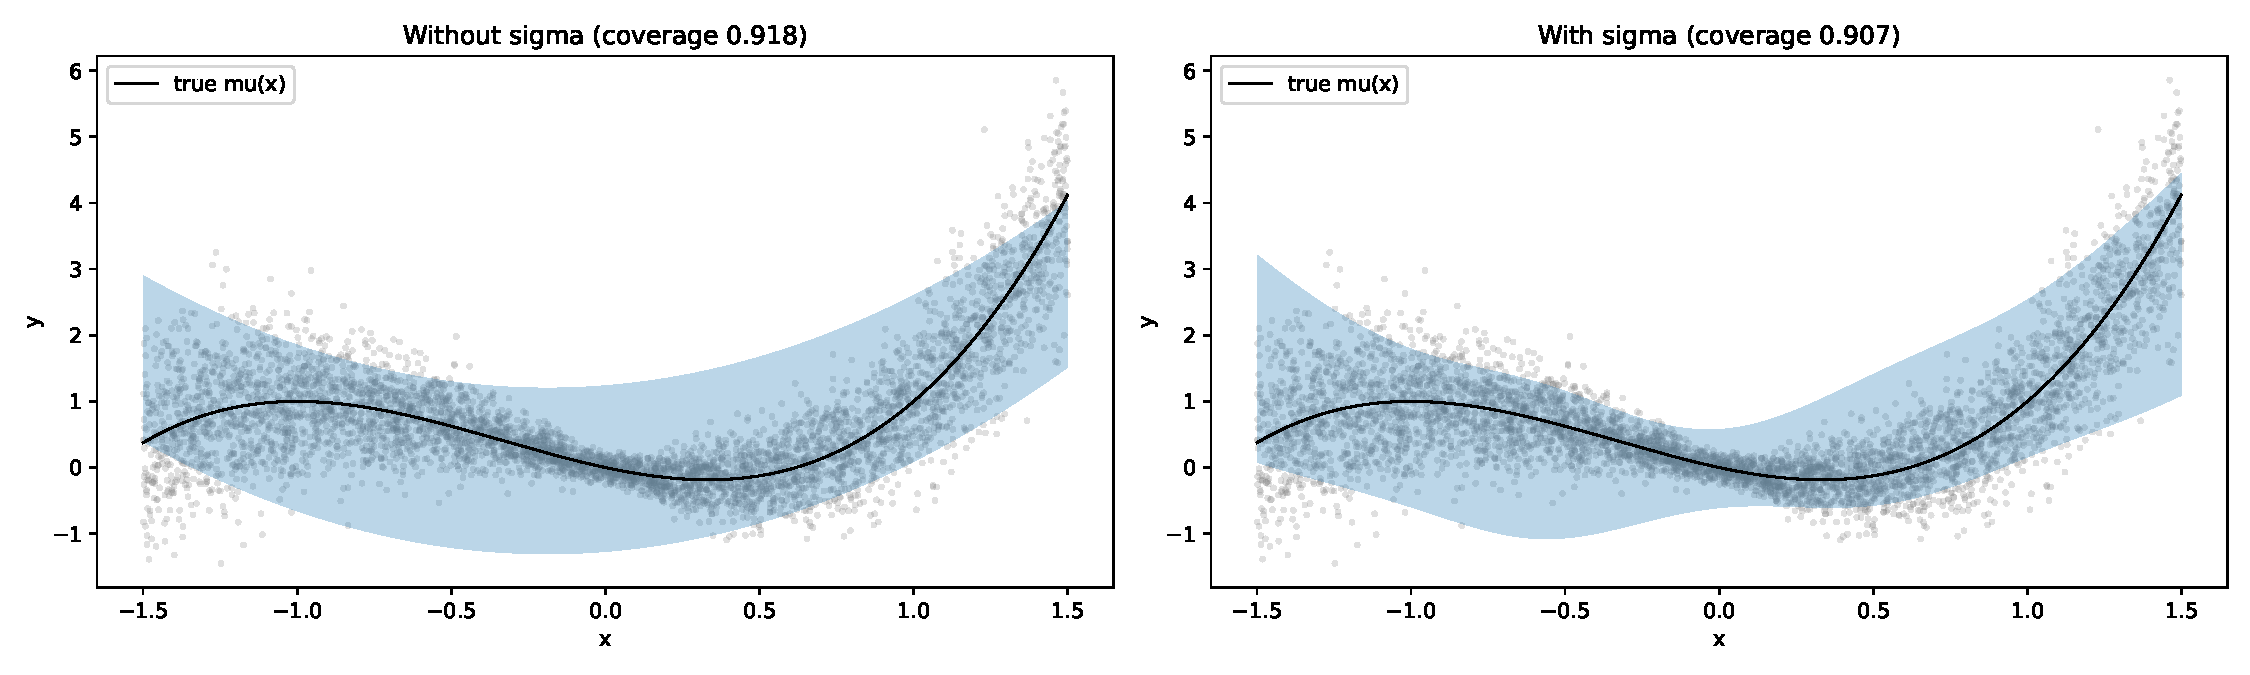
\includegraphics[width=0.95\textwidth]{split_conformal.pdf}
  \caption{Split conformal prediction regions with and without rescaling by
  $\hat{\sigma}_A(x)$. The data are generated from $Y=\mu(X)+\sigma(X)\varepsilon$
  with $\mu(x)=x^3-x$, $\sigma(x)=0.1+0.5\lvert x\rvert$,
  $X\sim\mathrm{Unif}[-1.5,1.5]$, and $\varepsilon\sim N(0,1)$. We use $500$ training
  data, $500$ calibration data, and $5000$ test data with $\alpha=0.1$, and
  $\hat{\mu}_A$ is the ordinary least squares estimator. The figures show the prediction regions without and with rescaling, respectively, together
  with the test data (gray points) and the true regression function (black line).}
  \label{fig:ch8-split-conformal-prediction}
\end{figure}

Figure~\ref{fig:ch8-split-conformal-prediction} illustrates the difference in the \emph{adaptivity} of the prediction regions. Without $\hat{\sigma}_A$, the prediction region has a constant width regardless of $x$ (left figure). With $\hat{\sigma}_A$, the width of the prediction region varies with $x$ (right figure). This shows that incorporating $\hat{\sigma}_A$ enables us to construct a prediction region that adapts to the heteroscedasticity of the data. More generally, accounting for heteroscedasticity is important not only in split conformal prediction but also in nonparametric regression.

\end{document}